\chapter{Meta Reinforcement Learning}%
\label{cha:meta_learning}

\lecture{20}{}{Meta Reinforcement Learning}

\section{¿Cuál es el problema?}%
\label{sec:_cuál_es_el_problema_}

Normalmente los agentes inteligentes suelen ser especialistas en una tarea, pero se quiere que
sean generalistas de tal forma que aprendan tareas de forma mucho más eficiente.

Por ejemplo un robot entrenado para hacer surf, no tiene por qué aprender de cero totalmente para
aprender a montar en moto.

\subsection{Enunciado del problema}%
\label{sub:enunciado_del_problema}

En el aprendizaje por refuerzo clásico, se tiene que aprender un MDP:
\begin{align}
    \theta*&=arg\max_\theta E_{\pi_\theta(\tau)}[R(\tau)]\\
           &=f_{RL}(M)
\end{align}
Donde $\theta$ son los parámetros de la política.

En Meta-RL, se tiene que aprender la \textbf{regla de adaptación}:
\begin{align}
    \label{eq:outerloop}
    \theta*&=arg\max_\theta \sum_{i=1}^n E_{\pi_{\phi_i}(\tau)}[R(\tau)]\\
    \label{eq:innerloop}
    \textrm{Donde } \phi_i&=f_\theta(M_i)
\end{align}
Donde $\theta$ no tiene por qué ser los parámetros de la política, si no que puede ser los
parámetros de la regla de adaptación. $M_i$ hace referencia al MDP de la tarea $i$.

La expresión \ref{eq:outerloop} se llama \textit{meta-training} o bucle externo y la
expresión \ref{eq:innerloop} se llama adaptación o bucle interno.

\subsection{Relación con las políticas orientadas a objetivos}%
\label{sub:relación_con_las_políticas_orientadas_a_objetivos}

En RL clásico se tiene un objetivo que queda representado por una función de recompensa. Por lo
que el agente entrena una política condicionada a un conocimiento del entorno para actuar
con respecto a ese objetivo.

En Meta-RL se pretende que el agente pueda actuar con nuevas funciones de recompensa o
dinámicas del entorno.

Las recompensas son una generalización estricta de los objetivos, ya que estos se pueden
representar con recompensas pero no al revés. Por ejemplo, no se puede representar como un
estado objetivo la función de recompensa que describe buscar mientras se evita, o
penalizaciones sobre las acciones.

\subsection{Adaptación}%
\label{sub:adaptación}

La adaptación consiste en:
\begin{itemize}
    \item Explorar: coleccionar los datos que mayor información den.
    \item Adaptar: Usar esos datos para obtener la política óptima.
\end{itemize}

\begin{algorithm}
    \caption{Boceto de un algoritmo Meta-RL general}
    Muestrar la tarea $i$ para recoger los datos $D_i$ \\
    Adaptar la política calculando $\phi_i=f(\theta.D_i)$ \\
    Recoger los datos $D_i'$ con la política adaptada $\pi_{\phi_i}$ \\
    Actualizar $\theta$ de acuerdo con $L(D_i',\phi_i)$
\end{algorithm}

De este algoritmo, los primeros 3 pasos conforman la adaptación y pueden realizarse más de
una vez en cada iteración. El cuarto paso en la práctica se suele actualizar sobre un
\textit{batch} de tareas.

Los diferentes algoritmos consisten en la elección de la función $f$ y la función de pérdida
$L$.

\section{Métodos solución}%
\label{sec:métodos_solución}

\subsection{Solución 1: Recurrencia}%
\label{sub:solución_1_recurrencia}

Se entrena una red neuronal recurrente con datos recogidos en forma de tuplas (estado,
acción, recompensa) con \textit{batches} de cada una de las tareas.

\begin{center}
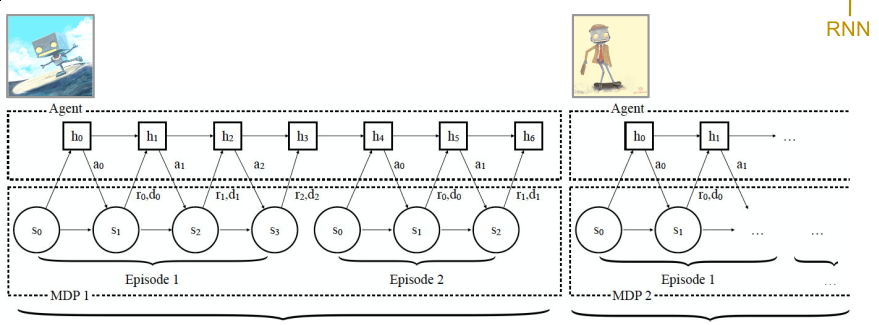
\includegraphics[width=0.8\textwidth]{figures/2020-07-25-175340_879x325_scrot.png}
\end{center}

\begin{algorithm}
    \caption{Boceto de recurrencia}
    \While{se entrene}{
        \For{i en tareas}{
            Inicializar el estado oculto $h_{0}=0$\\
            \For{t en pasos}{
                1. Muestrear 1 transición $D_i=D_i\cup\{(s_t,a_t,s_{t+1}, r_t)\}$ de
                $\pi_{h_t}$ \\
                2. Actualizar el estado oculto de la política $h_{t+1}=f_\theta(h_t,
                s_t, a_t, s_{t+1}, r_t)$
            }
        }
        Actualizar los parámetros de la política $\theta\gets\theta -
        \nabla_\theta\sum_iL_i(D_i,\pi_h)$
    }
\end{algorithm}

\begin{itemize}
    \item Ventajas: es general y expresivo ya que hay RNNs que pueden calcular cualquier
        función.
    \item Desventajas: no es consistente. Un modelo es consistente si converge a la
        política óptima dados los suficientes datos.
\end{itemize}

\subsection{Solución 2: Optimización}%
\label{sub:solución_2_optimización}

Extrapolando la idea de \textit{fine-tuning}, la idea de la optimización radica en aprender
una parametrización de modo que hacer fine-tuning para cada una de las tareas sea muy
rápido.

\begin{center}
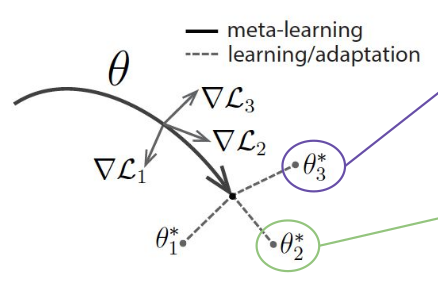
\includegraphics[width=0.4\textwidth]{figures/2020-07-25-180726_438x284_scrot.png}
\end{center}

En este caso, se tiene Policy Gradients tanto en la adaptación como en el bucle externo.

\begin{algorithm}
    \caption{Boceto de optimización}
    \While{se entrene}{
        \For{i en tareas}{
            Muestrar $k$ episodios $D_i=\{(s,a,s',r)\}_{1:k}$ de $\pi_\theta$ \\
            Calcular los parámetros adaptados $\phi_i=\theta-\alpha\nabla_\theta
            L_i(\pi_\theta,D_i)$.\\
            Muestrar $k$ episodios $D_i'=\{(s,a,s',r)\}_{1:k}$ de $\pi_\phi$
        }
        Actualizar los parámetros de la política
        $\theta\gets\theta-\nabla_\theta\sum_iL_i(D_i',\pi_{\phi_i})$.
    }
\end{algorithm}

Nótese que en el último paso, cuando se calcula el gradiente se está haciendo con
respecto al gradiente previo, por lo que se está calculando la derivada de segundo orden.

\begin{center}
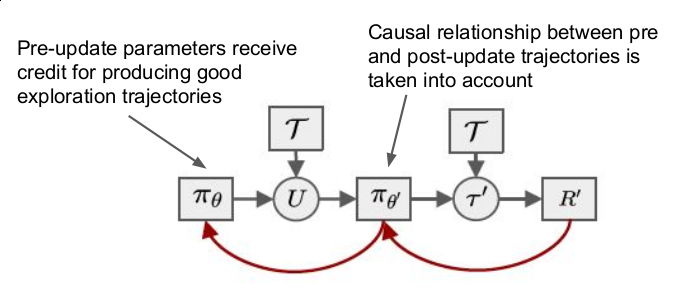
\includegraphics[width=0.6\textwidth]{figures/2020-07-25-183028_678x294_scrot.png}
\end{center}

\begin{itemize}
    \item Ventajas: es consistente ya que se está haciendo descenso por gradiente.
    \item Desventajas: no es tan expresivo. Sobretodo en entornos donde no se obtenga señal de recompensa
        la adaptación no cambiará la política, aunque los datos dan información sobre
        que estados se deben de evitar.
\end{itemize}

\section{Meta-RL en sistemas robóticos}%
\label{sec:meta_rl_en_sistemas_robóticos}

\subsection{Meta-imitation learning}%
\label{sub:meta_imitation_learning}

Se puede entrenar un agente para que aprenda a realizar una tarea a partir de una demostración
humana. Para el entrenamiento inicial se supone que se tienen pares de episodios tanto del
humano como del agentSe puede entrenar un agente para que aprenda a realizar una tarea a partir
de una demostración humana. Para el entrenamiento inicial se supone que se tienen pares de
episodios tanto del humano como del robot, realizando la misma acción. Al mostrar la nueva
acción del humano, el robot intentará imitarla.

\begin{center}
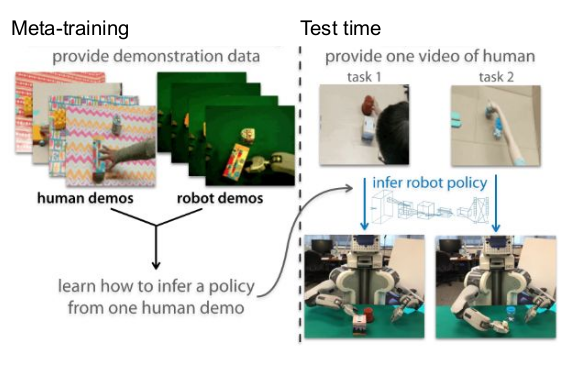
\includegraphics[width=.6\textwidth]{figures/2020-07-25-184423_582x365_scrot.png}
\end{center}

En este método se aprende la función de pérdida $f_\theta$.

\section{Meta-RL basado en modelo}%
\label{sec:meta_rl_basado_en_modelo}

En el aprendizaje basado en modelo, puede ocurrir que el entorno cambie ligeramente,
haciendo que el modelo aprendido sea inútil hasta que no se reentrene el agente, por lo que
es de interés que en vez de reentrenarlo con todos los datos para obtener el modelo se usen pocos
datos nuevos y se parta de los conocimientos ya obtenidos.

\begin{center}
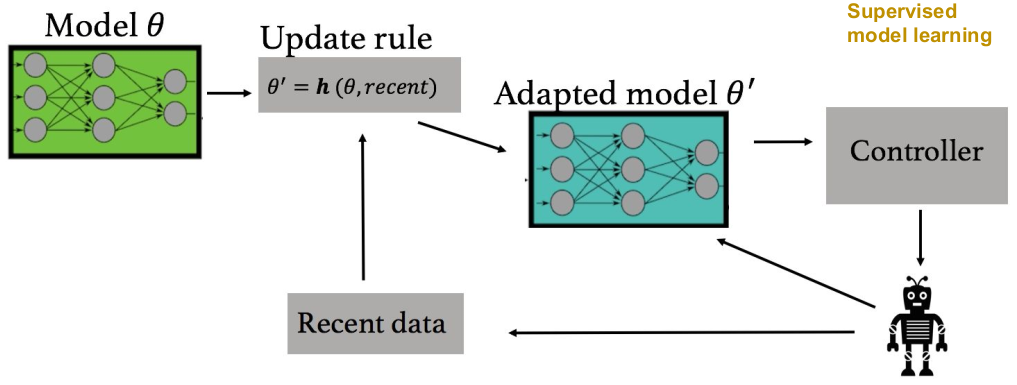
\includegraphics[width=.6\textwidth]{figures/2020-07-25-185920_1017x385_scrot.png}
\end{center}

\section{POMDP}%
\label{sec:pomdp}

\begin{center}
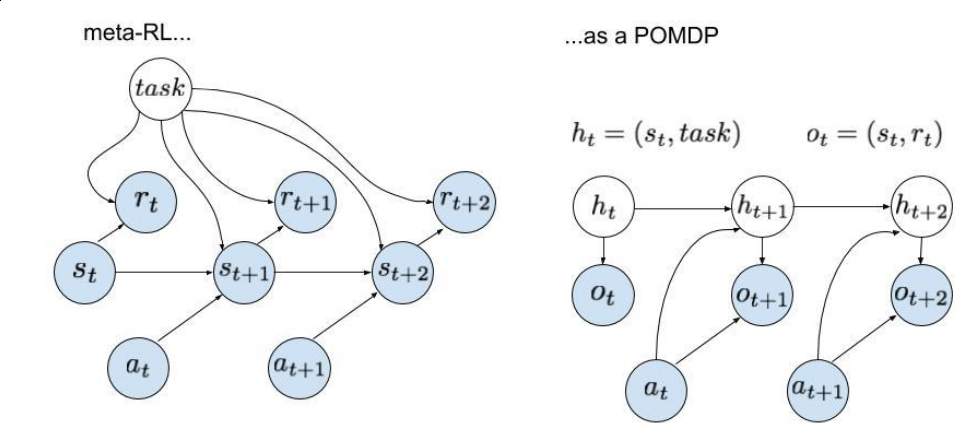
\includegraphics[width=.7\textwidth]{figures/2020-07-25-191537_980x428_scrot.png}
\end{center}

Hay dos aproximaciones para resolverlo:
\begin{itemize}
    \item RNN
    \item Estimación explícita del estado.
\end{itemize}
En este tema se va a tratar la segunda.

\begin{figure}
    \center
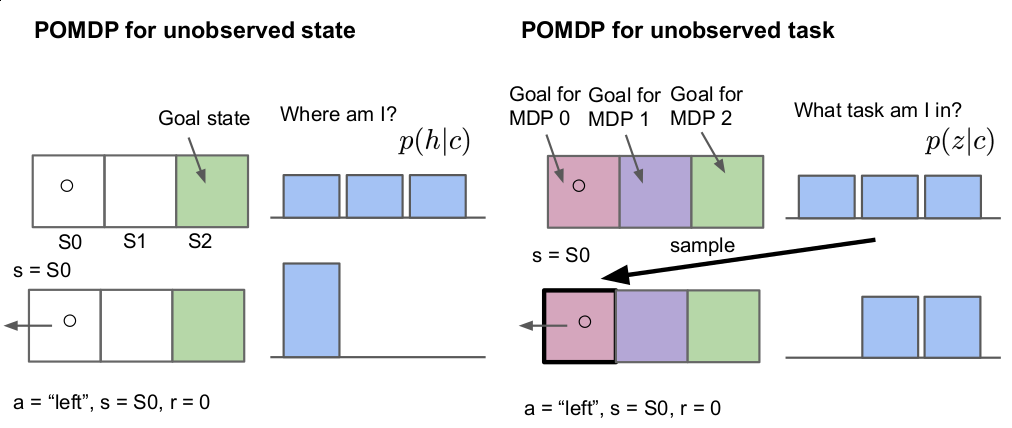
\includegraphics[width=.6\textwidth]{figures/2020-07-25-192831_1012x428_scrot.png}
\caption{Model belief over latent task variables}
\end{figure}

\section{Solución 3: Estados de creencia de tarea (task-belief states)}%
\label{sec:solución_3_estados_de_creencia_de_tarea_task_belief_states_}

Al entrenar para varias tareas, se va a ajustar un encoder estocástico para saber a que tarea
pertenecen los estados observados.

\begin{center}
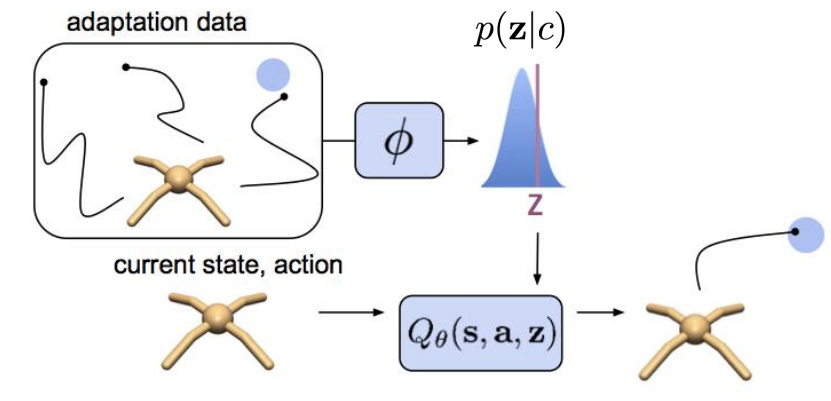
\includegraphics[width=.6\textwidth]{figures/2020-07-25-194057_831x401_scrot.png}
\end{center}

Se puede entrenar generando objetivos que se creen posibles, por ejemplo:
\begin{center}
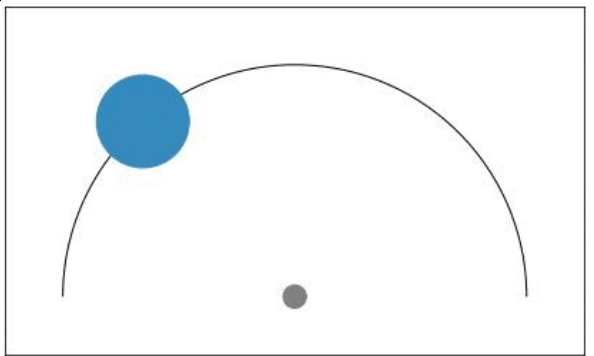
\includegraphics[width=.5\textwidth]{figures/2020-07-25-194442_594x356_scrot.png}
\end{center}
En este entorno se quiere ir del centro del círculo al círculo azul. Una vez el agente haya
aprendido a llegar, se pueden generar objetivos 'falsos' pensando que el círculo azul puede
estar en cualquier parte de la circunferencia, lo que hace que se aprenda muy rápido en caso
de que el área azul se mueva.

Aprender $p(z|c)$ es intratable, por lo que se hará uso de la inferencia variacional.

\begin{align}
    \E_{\tau}[\E_{z\sim q_{\phi}(z|c^\tau)}[R(\tau,z)+\beta
    D_{KL}(q_\phi(z|c^\tau)||p(z))]]
\end{align}

\begin{center}
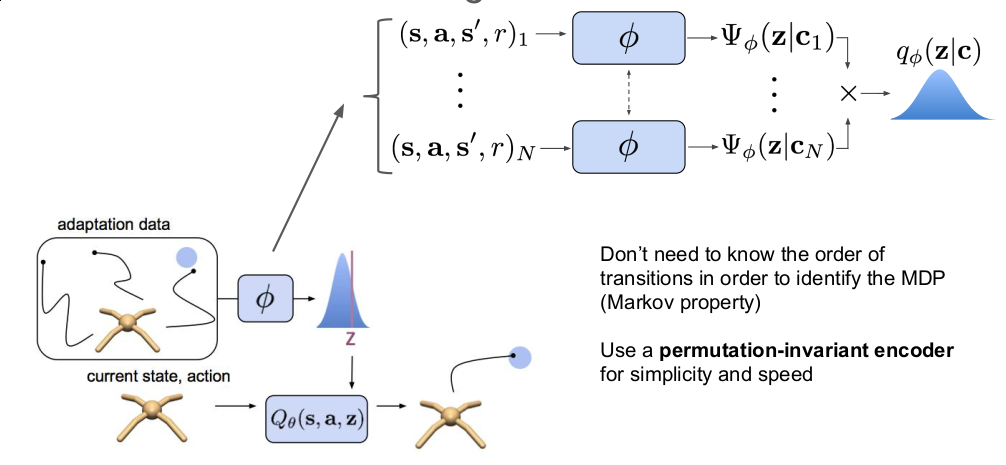
\includegraphics[width=.7\textwidth]{figures/2020-07-25-195700_1006x465_scrot.png}
\end{center}

\subsubsection{Soft Actor-Critic (SAC) + creencia de la tarea}%
\label{ssub:soft_actor_critic_sac_}

\begin{center}
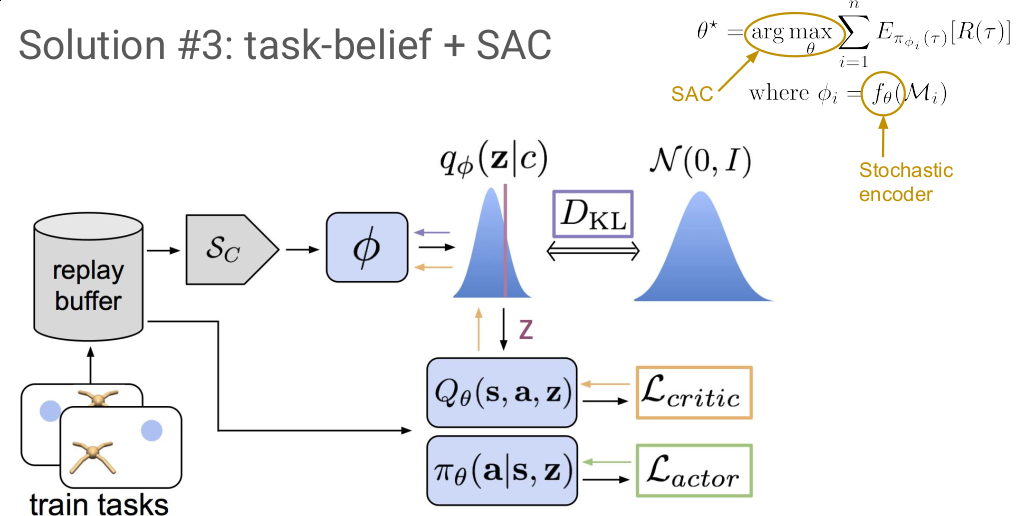
\includegraphics[width=.7\textwidth]{figures/2020-07-25-200536_1023x516_scrot.png}
\end{center}

\section{Resumen}%
\label{sec:resumen}

\begin{center}
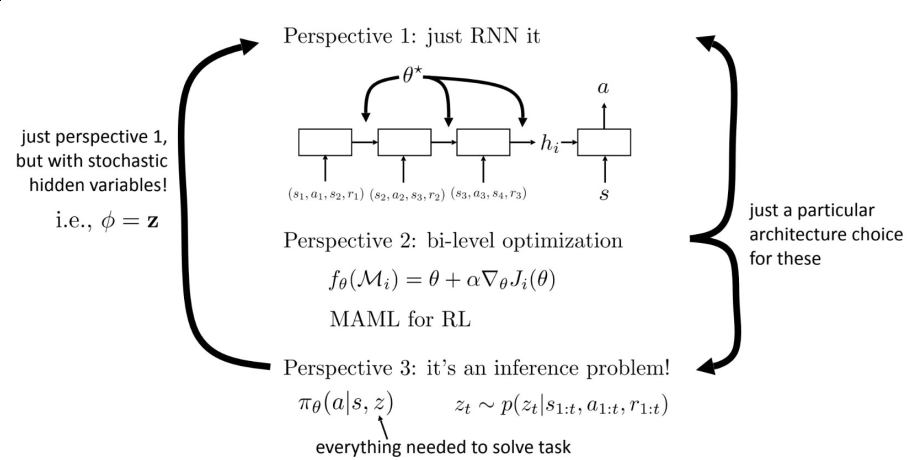
\includegraphics[width=.7\textwidth]{figures/2020-07-25-200918_910x460_scrot.png}
\end{center}

